% Appendices (formerly the separate supplementary material; supplement.tex is kept but no longer built)
\section{Inference latency variants}
\label{app:latency}
Every inference variant is timed end to end (BGR frame in, boxes out, batch 1, desktop RTX 4060 Laptop) and
re-scored, so speed-ups that cost accuracy are visible (PyTorch and TorchScript paths; the edge runtime uses ONNX Runtime~\cite{onnxruntime}).
\begin{table}[!htbp]
\centering
\caption{Inference variants on the \ImgsTest{} test frames ($1280{\times}720$, RTX 4060 Laptop, batch 1, pre- and
post-processing included). Median / p90 latency in ms and test \AP{} of each variant.}
\label{tab:lat}
\footnotesize
\setlength{\tabcolsep}{2.8pt}
\begin{tabular}{lccc}
\toprule
Variant & Median & p90 & \AP{} \\
\midrule
\multicolumn{4}{l}{\emph{\yolo{}}} \\
\quad Ultralytics predict FP32 (stock) & \LatYoloBase & \LatPnYoloBase & \LatApYoloBase \\
\quad Ultralytics predict FP16 & \LatYoloHalf & \LatPnYoloHalf & \LatApYoloHalf \\
\quad NMS-free head FP16 & \LatYoloNmsFree & \LatPnYoloNmsFree & \LatApYoloNmsFree \\
\quad NMS-free + GPU pre-proc + fused FP16 & \LatYoloNmsFreeFast & \LatPnYoloNmsFreeFast & \LatApYoloNmsFreeFast \\
\quad \textbf{GPU pre-proc + fused FP16 + GPU NMS} & \textbf{\LatYoloDep} & \LatPnYoloDep & \LatApYoloDep \\
\multicolumn{4}{l}{\emph{\rfdetr{}}} \\
\quad predict FP32 (stock) & \LatRfBase & \LatPnRfBase & \LatApRfBase \\
\quad FP32 + TorchScript & \LatRfTs & \LatPnRfTs & \LatApRfTs \\
\quad FP16 & \LatRfHalf & \LatPnRfHalf & \LatApRfHalf \\
\quad FP16 + TorchScript & \LatRfHalfTs & \LatPnRfHalfTs & \LatApRfHalfTs \\
\quad \textbf{FP16 + TorchScript + GPU pre-proc} & \textbf{\LatRfDep} & \LatPnRfDep & \LatApRfDep \\
\bottomrule
\end{tabular}
\end{table}

\begin{figure}[!htbp]
\centering
\figif{fig_latency.pdf}{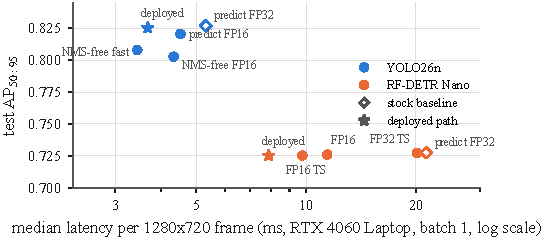
\includegraphics[width=\columnwidth]{figures/fig_latency.pdf}}
\caption{Latency vs.\ test \AP{} of the inference variants of Table~\ref{tab:lat} (stars: deployed paths).}
\label{fig:lat}
\end{figure}

\figif{fig_qualitative.png}{%
\begin{figure*}[!htbp]
\centering
\includegraphics[width=0.86\textwidth]{figures/fig_qualitative.png}
\caption{Test frames: teacher pseudo-GT (left), fine-tuned \yolo{} (centre) and fine-tuned \rfdetr{} (right) at
their valid-optimal thresholds; titles give the number of boxes.}
\label{fig:qual}
\end{figure*}}

\section{Campus case study (offline, teacher detector)}
\label{app:campus}
% from the submitted version (lines 697-737), revised
%-----------------------------------------------------------------------------------------------------
\label{sec:campus}
To test transfer to a new domain we analysed two $\sim$200\,s, 1080p phone videos of a university campus. Nothing
here needs real time, so the teacher detector YOLO26x at 1280\,px is used with BoT-SORT (ReID and motion
compensation); broken tracks are re-joined offline when motion, box size, colours and predicted attributes agree.
Two attribute heads (uniform vs.\ non-uniform, gender) are logistic-regression probes on DINOv2 features of the
RF-DETR-L backbone plus colour histograms, trained on 200 hand-labelled tracks and evaluated on 100 disjoint
random tracks; they abstain when the mean probability is within 0.35--0.65. Table~\ref{tab:campus} and
Fig.~\ref{fig:campus} summarise the outputs. Held out per person, the probes reach \PrUniAcc{}
\ci{\PrUniLo}{\PrUniHi} accuracy for dress (\PrUniCorrect/\PrUniAnswered, coverage \PrUniCov) and \PrGenAcc{}
\ci{\PrGenLo}{\PrGenHi} for gender (\PrGenCorrect/\PrGenAnswered, coverage \PrGenCov). The hand labels were
produced by the authors' AI assistant from the crops, not by independent annotators, and gender is predicted from
appearance (the uniform is gendered); it is reported only as an aggregate.

\begin{table}[!htbp]
\centering
\caption{Campus case study (YOLO26x + BoT-SORT + stitching; attributes over people with a usable crop).}
\label{tab:campus}
\footnotesize
\setlength{\tabcolsep}{2.4pt}
\begin{tabular}{lcc}
\toprule
 & video 1 & video 2 \\
\midrule
Track IDs $\rightarrow$ kept $\rightarrow$ people & \CpOneRaw{} $\rightarrow$ \CpOneKept{} $\rightarrow$ \CpOnePeople & \CpTwoRaw{} $\rightarrow$ \CpTwoKept{} $\rightarrow$ \CpTwoPeople \\
In frame, mean / peak & \CpOneMean{} / \CpOnePeak & \CpTwoMean{} / \CpTwoPeak \\
Crossings (R$\rightarrow$L/L$\rightarrow$R) & \CpOneCross{} (\CpOneCrossRl/\CpOneCrossLr) & \CpTwoCross{} (\CpTwoCrossRl/\CpTwoCrossLr) \\
Median time in view (s) & \CpOneDwell & \CpTwoDwell \\
Gender m / f / unsure & \CpOneMale{} / \CpOneFemale{} / \CpOneGUnsure & \CpTwoMale{} / \CpTwoFemale{} / \CpTwoGUnsure \\
Dress unif. / non-u. / unsure & \CpOneUniform{} / \CpOneNonUniform{} / \CpOneDUnsure & \CpTwoUniform{} / \CpTwoNonUniform{} / \CpTwoDUnsure \\
\bottomrule
\end{tabular}
\end{table}

\begin{figure}[!htbp]
\centering
\figif{fig_campus.pdf}{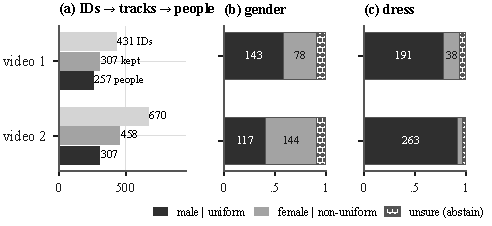
\includegraphics[width=\columnwidth]{figures/fig_campus.pdf}}
\caption{Campus case study: (a) counting funnel from raw track IDs to stitched people; (b, c) attribute shares.}
\label{fig:campus}
\end{figure}


% moved from the main paper to save space
\section{Additional figures}
\label{app:figs}
\begin{figure}[!htbp]
\centering
\figif{fig_pr.pdf}{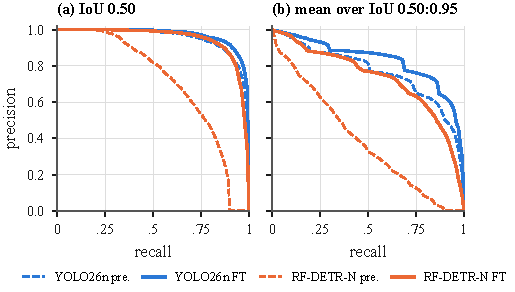
\includegraphics[width=\columnwidth]{figures/fig_pr.pdf}}
\caption{aa1 test precision--recall curves (dashed: COCO-pretrained, solid: fine-tuned).}
\label{fig:pr}
\end{figure}
\begin{figure}[!htbp]
\centering
\figif{fig_selection.pdf}{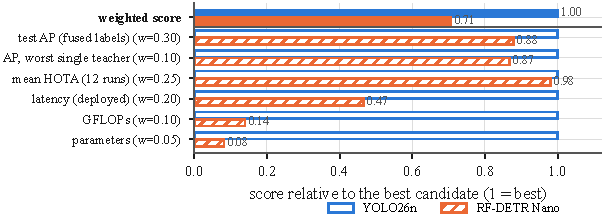
\includegraphics[width=\columnwidth]{figures/fig_selection.pdf}}
\caption{Normalised decision criteria (1 = best candidate) and weighted score.}
\label{fig:sel}
\end{figure}
\begin{figure}[!htbp]
\centering
\figif{fig_edge.pdf}{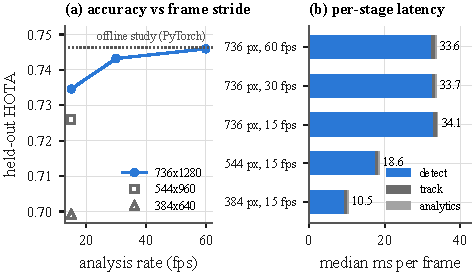
\includegraphics[width=\columnwidth]{figures/fig_edge.pdf}}
\caption{Deployed runtime: (a) held-out HOTA vs.\ analysis rate and input size; (b) median per-stage latency
(desktop CPU ONNX Runtime, not TensorRT).}
\label{fig:edge}
\end{figure}
\section{E2: zero-shot attributes}
\label{app:e2}
\ifHaveVLMETwo
\textbf{E2: zero-shot attributes.} On the held-out campus test tracks, the VLM's zero-shot uniform/gender votes
(three crops per track) are compared with the trained linear probes of Sec.~\ref{sec:campus}. Per track,
dress accuracy is \EtVlmAccUni{} \ci{\EtVlmLoUni}{\EtVlmHiUni} (Wilson CI~\cite{wilson1927}) for the VLM vs.\ \EtProbeAccUni{} for the probe
(coverage \EtVlmCovUni{} vs.\ \EtProbeCovUni), and gender \EtVlmAccGen{} vs.\ \EtProbeAccGen; on the tracks both
answered, an exact McNemar test~\cite{mcnemar1947} gives \EtMcPUni{} and \EtMcPGen. Zero-shot description is thus
competitive with trained probes here.
\fi

\section{Full statistics and safety tables}
\label{app:stats}
Tables~\ref{tab:ci_aa1} and~\ref{tab:ci_ho} give the 95\% \AP{} intervals of all four detectors under every
resampling scheme of Sec.~\ref{sec:stats}: the i.i.d.\ frame bootstrap, the circular block bootstrap (CBB) with
2.5, 5 and 10\,s blocks, the moving block bootstrap (MBB) and CBB with the Politis--White automatic block length.
Table~\ref{tab:e6cat} gives the per-category counts behind Fig.~\ref{fig:safety}.
\begin{table}[!htbp]
\centering
\caption{95\% CIs of \AP{} on the aa1 test split under every resampling scheme ($B{=}\TcB$).}
\label{tab:ci_aa1}
\scriptsize\setlength{\tabcolsep}{1.5pt}
\begin{tabular}{lcccc}
\toprule
Scheme & YOLO pre. & YOLO FT & RF-DETR pre. & RF-DETR FT \\
\midrule
i.i.d. & \ci{\TcAaIidYoloPtLo}{\TcAaIidYoloPtHi} & \ci{\TcAaIidYoloFtLo}{\TcAaIidYoloFtHi} & \ci{\TcAaIidRfPtLo}{\TcAaIidRfPtHi} & \ci{\TcAaIidRfFtLo}{\TcAaIidRfFtHi} \\
CBB 2.5\,s & \ci{\TcAaCbbAYoloPtLo}{\TcAaCbbAYoloPtHi} & \ci{\TcAaCbbAYoloFtLo}{\TcAaCbbAYoloFtHi} & \ci{\TcAaCbbARfPtLo}{\TcAaCbbARfPtHi} & \ci{\TcAaCbbARfFtLo}{\TcAaCbbARfFtHi} \\
CBB 5\,s & \ci{\TcAaCbbBYoloPtLo}{\TcAaCbbBYoloPtHi} & \ci{\TcAaCbbBYoloFtLo}{\TcAaCbbBYoloFtHi} & \ci{\TcAaCbbBRfPtLo}{\TcAaCbbBRfPtHi} & \ci{\TcAaCbbBRfFtLo}{\TcAaCbbBRfFtHi} \\
CBB 10\,s & \ci{\TcAaCbbCYoloPtLo}{\TcAaCbbCYoloPtHi} & \ci{\TcAaCbbCYoloFtLo}{\TcAaCbbCYoloFtHi} & \ci{\TcAaCbbCRfPtLo}{\TcAaCbbCRfPtHi} & \ci{\TcAaCbbCRfFtLo}{\TcAaCbbCRfFtHi} \\
MBB 5\,s & \ci{\TcAaMbbBYoloPtLo}{\TcAaMbbBYoloPtHi} & \ci{\TcAaMbbBYoloFtLo}{\TcAaMbbBYoloFtHi} & \ci{\TcAaMbbBRfPtLo}{\TcAaMbbBRfPtHi} & \ci{\TcAaMbbBRfFtLo}{\TcAaMbbBRfFtHi} \\
CBB auto & \ci{\TcAaCbbAutoYoloPtLo}{\TcAaCbbAutoYoloPtHi} & \ci{\TcAaCbbAutoYoloFtLo}{\TcAaCbbAutoYoloFtHi} & \ci{\TcAaCbbAutoRfPtLo}{\TcAaCbbAutoRfPtHi} & \ci{\TcAaCbbAutoRfFtLo}{\TcAaCbbAutoRfFtHi} \\
\bottomrule
\end{tabular}
\end{table}
\begin{table}[!htbp]
\centering
\caption{95\% CIs of \AP{} on the held-out test1 video under every resampling scheme ($B{=}\TcB$).}
\label{tab:ci_ho}
\scriptsize\setlength{\tabcolsep}{1.5pt}
\begin{tabular}{lcccc}
\toprule
Scheme & YOLO pre. & YOLO FT & RF-DETR pre. & RF-DETR FT \\
\midrule
i.i.d. & \ci{\TcHoIidYoloPtLo}{\TcHoIidYoloPtHi} & \ci{\TcHoIidYoloFtLo}{\TcHoIidYoloFtHi} & \ci{\TcHoIidRfPtLo}{\TcHoIidRfPtHi} & \ci{\TcHoIidRfFtLo}{\TcHoIidRfFtHi} \\
CBB 2.5\,s & \ci{\TcHoCbbAYoloPtLo}{\TcHoCbbAYoloPtHi} & \ci{\TcHoCbbAYoloFtLo}{\TcHoCbbAYoloFtHi} & \ci{\TcHoCbbARfPtLo}{\TcHoCbbARfPtHi} & \ci{\TcHoCbbARfFtLo}{\TcHoCbbARfFtHi} \\
CBB 5\,s & \ci{\TcHoCbbBYoloPtLo}{\TcHoCbbBYoloPtHi} & \ci{\TcHoCbbBYoloFtLo}{\TcHoCbbBYoloFtHi} & \ci{\TcHoCbbBRfPtLo}{\TcHoCbbBRfPtHi} & \ci{\TcHoCbbBRfFtLo}{\TcHoCbbBRfFtHi} \\
CBB 10\,s & \ci{\TcHoCbbCYoloPtLo}{\TcHoCbbCYoloPtHi} & \ci{\TcHoCbbCYoloFtLo}{\TcHoCbbCYoloFtHi} & \ci{\TcHoCbbCRfPtLo}{\TcHoCbbCRfPtHi} & \ci{\TcHoCbbCRfFtLo}{\TcHoCbbCRfFtHi} \\
MBB 5\,s & \ci{\TcHoMbbBYoloPtLo}{\TcHoMbbBYoloPtHi} & \ci{\TcHoMbbBYoloFtLo}{\TcHoMbbBYoloFtHi} & \ci{\TcHoMbbBRfPtLo}{\TcHoMbbBRfPtHi} & \ci{\TcHoMbbBRfFtLo}{\TcHoMbbBRfFtHi} \\
CBB auto & \ci{\TcHoCbbAutoYoloPtLo}{\TcHoCbbAutoYoloPtHi} & \ci{\TcHoCbbAutoYoloFtLo}{\TcHoCbbAutoYoloFtHi} & \ci{\TcHoCbbAutoRfPtLo}{\TcHoCbbAutoRfPtHi} & \ci{\TcHoCbbAutoRfFtLo}{\TcHoCbbAutoRfFtHi} \\
\bottomrule
\end{tabular}
\end{table}
\begin{table}[!htbp]
\centering
\caption{E6 per category: cases handled safely (authorised: carried out correctly), out of $n$.}
\label{tab:e6cat}
\scriptsize\setlength{\tabcolsep}{2.5pt}
\begin{tabular}{lcccc}
\toprule
Category & $n$ & model only & + guardrails & + policy \\
\midrule
authorised (success) & \SfNAuth & \SfMoAuthK & \SfGrAuthK & \SfPoAuthK \\
ambiguous & \SfNAmb & \SfMoAmbK & \SfGrAmbK & \SfPoAmbK \\
conflicting & \SfNConf & \SfMoConfK & \SfGrConfK & \SfPoConfK \\
unauthorised role & \SfNUnauth & \SfMoUnauthK & \SfGrUnauthK & \SfPoUnauthK \\
malformed / out of range & \SfNMalf & \SfMoMalfK & \SfGrMalfK & \SfPoMalfK \\
alert-disabling & \SfNDis & \SfMoDisK & \SfGrDisK & \SfPoDisK \\
direct injection & \SfNInj & \SfMoInjK & \SfGrInjK & \SfPoInjK \\
frame-text injection & \SfNFrame & \SfMoFrameK & \SfGrFrameK & \SfPoFrameK \\
tool-result injection & \SfNTool & \SfMoToolK & \SfGrToolK & \SfPoToolK \\
multi-turn escalation & \SfNMulti & \SfMoMultiK & \SfGrMultiK & \SfPoMultiK \\
\bottomrule
\end{tabular}
\end{table}

